%==============================================================================
% Plug-and-Play Whole-Body Contact Estimation
%   A controller-agnostic proprioceptive force estimator for humanoids
% Target: IEEE-RAS Humanoids 2026 (IEEEtran conference, two-column, 10pt)
% Build : pdflatex -> bibtex -> pdflatex -> pdflatex
% NOTE  : separate from the ProACT (active-sensing) paper.
% FIGURES: all \includegraphics point to figs/*.pdf that are NOT yet generated;
%          each is wrapped in \todofig{...} describing what to plot. Search
%          "TODO-FIG" to find every figure that still needs to be produced.
%==============================================================================
\documentclass[conference]{IEEEtran}
\IEEEoverridecommandlockouts

\usepackage{cite}
\usepackage{amsmath,amssymb,amsfonts}
\usepackage{graphicx}
\usepackage{booktabs}
\usepackage{multirow}
\usepackage{textcomp}
\usepackage{xcolor}
\usepackage{url}
\usepackage[hidelinks]{hyperref}
\usepackage{tikz}
\usetikzlibrary{arrows.meta,positioning,fit,backgrounds}

\newcommand{\Fext}{\mathbf{F}_{\mathrm{ext}}}
\newcommand{\tauext}{\boldsymbol{\tau}_{\mathrm{ext}}}

% Placeholder box for a figure that still needs to be produced. Replace the
% whole \todofig{...} with \includegraphics{...} once figs/<name>.pdf exists.
\newcommand{\todofig}[2]{%
  \fbox{\parbox[c][#1][c]{0.96\linewidth}{\centering\footnotesize\color{red}%
  \textbf{[TODO-FIG: #2]}}}}

\begin{document}

\title{Plug-and-Play Whole-Body Contact Estimation:\\
       A Controller-Agnostic Proprioceptive Force Estimator for Humanoids}

\author{
\IEEEauthorblockN{Anonymous Author(s)}
\IEEEauthorblockA{\textit{Affiliation} \\ \textit{Institution}\\
City, Country \\ email@domain}
}

\maketitle

\begin{figure*}[t]
\centering
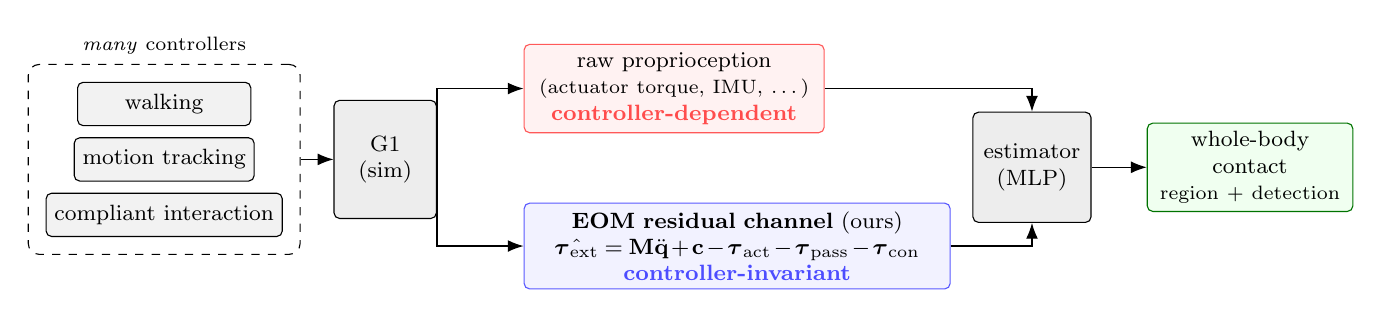
\begin{tikzpicture}[
  font=\footnotesize, >={Latex[length=2mm]}, node distance=8mm,
  box/.style={draw, rounded corners=2pt, align=center, inner sep=3pt},
  ctrl/.style={box, fill=black!5, minimum width=22mm, minimum height=5.5mm},
  dep/.style={box, draw=red!65, fill=red!5, align=center, text width=36mm},
  inv/.style={box, draw=blue!65, fill=blue!5, align=center, text width=52mm},
  est/.style={box, fill=black!7, minimum width=15mm, minimum height=14mm},
  obox/.style={box, draw=green!45!black, fill=green!6, text width=24mm}]
% controller bank
\node[ctrl] (c1) {walking};
\node[ctrl, below=1.4mm of c1] (c2) {motion tracking};
\node[ctrl, below=1.4mm of c2] (c3) {compliant interaction};
\begin{scope}[on background layer]
\node[draw, dashed, rounded corners, fit=(c1)(c2)(c3), inner sep=2.2mm,
      label=above:{\scriptsize \emph{many} controllers}] (bank) {};
\end{scope}
% robot
\node[box, fill=black!7, right=10mm of c2, minimum width=13mm,
      minimum height=15mm] (robot) {G1\\(sim)};
% two channels
\node[dep, right=11mm of robot, yshift=9mm]
      (dep) {raw proprioception\\{\scriptsize (actuator torque, IMU, \ldots)}\\
              \textcolor{red!70}{\textbf{controller-dependent}}};
\node[inv, right=11mm of robot, yshift=-11mm]
      (inv) {\textbf{EOM residual channel} (ours)\\
              $\hat{\tauext}\!=\!\mathbf{M}\ddot{\mathbf q}\!+\!\mathbf c
               \!-\!\boldsymbol\tau_{\mathrm{act}}
               \!-\!\boldsymbol\tau_{\mathrm{pass}}
               \!-\!\boldsymbol\tau_{\mathrm{con}}$\\
              \textcolor{blue!70}{\textbf{controller-invariant}}};
% estimator + output
\node[est, right=68mm of robot, yshift=-1mm] (mlp) {estimator\\(MLP)};
\node[obox, right=7mm of mlp] (o) {whole-body contact\\{\scriptsize region + detection}};
% arrows
\draw[->] (bank.east) -- (robot.west);
\draw[->] (robot.east) |- (dep.west);
\draw[->] (robot.east) |- (inv.west);
\draw[->] (dep.east) -| (mlp.north);
\draw[->] (inv.east) -| (mlp.south);
\draw[->] (mlp.east) -- (o.west);
\end{tikzpicture}
\caption{\textbf{Plug-and-play contact estimation.} A humanoid runs many
controllers, but a proprioceptive contact estimator is trained under one. The raw
proprioception an end-to-end estimator relies on is \textcolor{red!70}{controller-dependent}
(its actuator-torque distribution shifts with the control law), so the estimator
does not transfer. We add a \textcolor{blue!70}{controller-invariant} residual
channel recovered from the equation of motion --- it depends only on measured
motion and the model, not on how the torque was produced --- which lets one
estimator plug into unseen controllers and, by subtracting the ground reaction,
also un-masks the legs.}
\label{fig:overview}
\end{figure*}

\begin{abstract}
A humanoid can estimate external contact forces over its whole body from
proprioception alone, without force/torque sensors. But such estimators are
trained end-to-end under \emph{one} controller, whereas a deployed humanoid runs
\emph{many} --- walking, several motion-tracking policies, compliant-interaction
policies. A contact estimator would be far more useful as a \emph{plug-and-play}
module that drops onto any of them unchanged. We show the standard recipe does
not transfer: trained on one controller and evaluated across seven others
(kp/kd-scaled variants under an identical ground-truth force protocol),
worst-case region localization falls to $0.42$ and detection precision collapses
to $0.53$ --- a different torque baseline is read as contact. We trace this to the
estimator leaning on the raw actuator-torque channel, whose distribution the
controller sets, and introduce a \emph{controller-invariant residual channel}: a
per-joint external-torque estimate from the equation of motion, depending only on
the measured motion and the known model. It nearly eliminates the gap
(worst-case region accuracy $0.42\!\to\!0.91$, precision $0.53\!\to\!0.97$ across
all seven controllers). The same channel unexpectedly solves the hardest
localization case: because it subtracts the ground reaction it removes
double-support \emph{stance masking}, raising leg-region recall from $0.56$ to
$0.89$. Finally we make the channel hardware-realizable: the only
simulation-privileged term is the ground reaction; dropping it leaves the upper
body fully controller-invariant from proprioception alone ($0.94$), and supplying
the ground reaction from a foot force estimate recovers the legs, degrading
gracefully with estimation error ($0.79$ at $25\%$ error). All experiments are in
simulation on a Unitree G1.
\end{abstract}

%==============================================================================
\section{Introduction}
Physical interaction is central to what we want humanoids to do: leaning on a
wall, being pushed, carrying a load, working in clutter. Detecting and localizing
external contact is a prerequisite, and while dedicated skin or force/torque
(F/T) sensing remains rare on full humanoids, recent results show that a
surprising amount of contact information is recoverable from
\emph{proprioception alone} --- joint positions, velocities, actuator torques,
and IMU. SixthSense~\cite{sixthsense}, for example, regresses a per-link wrench
field over the whole body of a Unitree G1 from a short proprioceptive history.

These estimators are learned end-to-end, and crucially they are trained on data
collected under \emph{one} controller --- the policy driving the robot during
collection. In practice a humanoid is not one controller: it runs a walking
policy, one or more motion-tracking policies, a compliant-interaction
policy~\cite{gentlehumanoid}, and so on. A contact estimator would be most
valuable as an \emph{infrastructure} component --- a plug-and-play module that
reads only proprioception and drops onto \emph{any} of these controllers without
re-collecting data and re-training (Fig.~\ref{fig:overview}). Whether current
estimators have this property
has, to our knowledge, never been tested: the estimator and its single controller
are always evaluated together.

This paper isolates and answers that question, and finds that the answer changes
what such an estimator should take as input. Our contributions are:
\begin{enumerate}
\item We define and measure the \emph{cross-controller generalization gap}. Using
seven PD-gain-scaled controller variants under an identical ground-truth contact
protocol (the controller is the only variable), a leave-one-out study shows the
gap is large: worst-case region localization $0.42$ and detection precision
$0.53$ on unseen controllers (Sec.~\ref{sec:gap}).
\item We identify the cause --- the estimator leans on the raw actuator-torque
channel, whose distribution the controller sets --- and introduce a
\emph{controller-invariant residual channel} from the equation of motion. It
nearly closes the gap (worst-case region accuracy $0.91$, precision $0.97$),
robustly across all seven controllers including extreme extrapolation
(Sec.~\ref{sec:method},~\ref{sec:robust}).
\item We show the same channel \emph{solves the legs}: subtracting the ground
reaction removes double-support stance masking, raising leg-region recall
$0.56\!\to\!0.89$, near arm level (Sec.~\ref{sec:legs}).
\item We make the channel \emph{hardware-realizable}: its only
simulation-privileged term is the ground reaction. Without it the upper body is
still fully controller-invariant from proprioception alone ($0.94$); with a foot
force estimate the legs are recovered and degrade gracefully with estimation
error (Sec.~\ref{sec:realize}).
\end{enumerate}
We are explicit about what a simulation study establishes
(Sec.~\ref{sec:limits}): ``different controller'' is emulated by gain scaling, not
by genuinely different networks, so our gap is a \emph{lower bound}.

%==============================================================================
\section{Related Work}
\textbf{Proprioceptive contact/force estimation.} SixthSense~\cite{sixthsense}
estimates a whole-body per-link wrench field on a real G1 from a $\sim$1\,s
proprioceptive window, and is the closest system to ours; it targets transient
pushes and is trained and evaluated within a single control pipeline. Classical
\emph{momentum observers}~\cite{deluca2006momentum} estimate external joint
torques from generalized momentum without joint accelerations, independent of the
control law by construction; MOB-Net~\cite{mobnet} learns a floating-base
momentum observer for whole-body wrench estimation, and FACTR\,2~\cite{factr2}
self-supervises a free-space external-torque model for label-free, sensorless
force estimation.
Our residual channel is a learning \emph{input} in the same spirit --- a
physics-derived, controller-invariant signal --- rather than a standalone
estimator, and we study specifically its effect on \emph{cross-controller}
transfer, and its side effect on leg observability.

\textbf{Compliant humanoid interaction.} GentleHumanoid~\cite{gentlehumanoid}
learns upper-body compliance for contact-rich interaction using an impedance
formulation~\cite{hogan1985impedance} and proprioception-only deployment; it
solves how to \emph{respond} softly to contact but does not localize it. A
plug-and-play estimator is a natural complement: it would let such a controller
know \emph{where} it is being touched.

\textbf{Randomization for transfer.} Domain/dynamics
randomization~\cite{tobin2017domainrand} trains across a distribution of
environment parameters to obtain robustness to the sim-to-real gap. We use the
analogous idea along a new axis --- the \emph{downstream controller} --- and
compare it against, and combine it with, the physics-based residual channel.

%==============================================================================
\section{The Cross-Controller Generalization Gap}
\label{sec:gap}

\subsection{Setup}
We use a Unitree G1 in MuJoCo~\cite{todorov2012mujoco}, driven by a fixed,
exported standing/motion-tracking policy through a position-PD actuator, in a
sim-to-sim pipeline that reproduces the training-time observation and action
semantics. External forces follow a scripted protocol (rest / ramp / hold /
release, $|\Fext|\!\in\![10,40]$\,N, isotropic direction, one of $24$ candidate
links per cycle) giving exact ground-truth contact location and force; a frame is
labeled \emph{contact} when $|\Fext|>5$\,N. The estimator reads a $6$-step
proprioceptive window (applied torque, joint-position history, angular velocity,
projected gravity, past actions; $320$ dims/frame) and has two heads: a detection
logit and a $5$-region classifier (left/right arm, left/right leg, trunk). We
report detection precision/recall/F1 and region-localization accuracy on contact
frames (regAcc).

\textbf{Emulating different controllers.} To vary the controller while holding
everything else fixed, we scale the deploy PD gains, which enter the actuator
torque $\boldsymbol{\tau}=k_p(\mathbf{q}_{\mathrm{des}}-\mathbf{q})-k_d\dot{\mathbf{q}}$
directly --- exactly the channel a different downstream policy would shift. We use
\textbf{seven} controllers spanning $k_p\!\in\![0.4,2.0]\times$ and
$k_d\!\in\![0.5,1.5]\times$ nominal, independently varied (Table~\ref{tab:ctrl}),
and collect $360$k frames each.

\begin{table}[t]
\centering
\caption{The seven controller variants (PD-gain scale vs.\ nominal).}
\label{tab:ctrl}
\small
\begin{tabular}{lccccccc}
\toprule
 & base & soft & stiff & soft-ud & v-stiff & under-d & over-d \\
\midrule
$k_p$ & 1.0 & 0.6 & 1.5 & 0.4 & 2.0 & 1.0 & 0.7 \\
$k_d$ & 1.0 & 0.8 & 1.2 & 0.7 & 1.5 & 0.5 & 1.5 \\
\bottomrule
\end{tabular}
\end{table}

\subsection{Result: the gap is large}
Table~\ref{tab:main} (``proprioception'' rows) and Fig.~\ref{fig:gap} report a
leave-one-out study: train on six controllers, evaluate on the held-out unseen
one. Even with this randomization, raw proprioception is fragile --- worst-case
region accuracy $0.42$ and detection precision $0.53$ (the extreme-soft
controller, an extrapolation below the training range), and only $0.65$ mean
accuracy. Under a different torque baseline the estimator reads contact-free
stance as contact. A naive end-to-end estimator therefore does \emph{not} plug and
play, and because gain scaling is a comparatively small perturbation of the torque
distribution, the gap for a genuinely different policy can only be larger.

\begin{figure}[t]
\centering
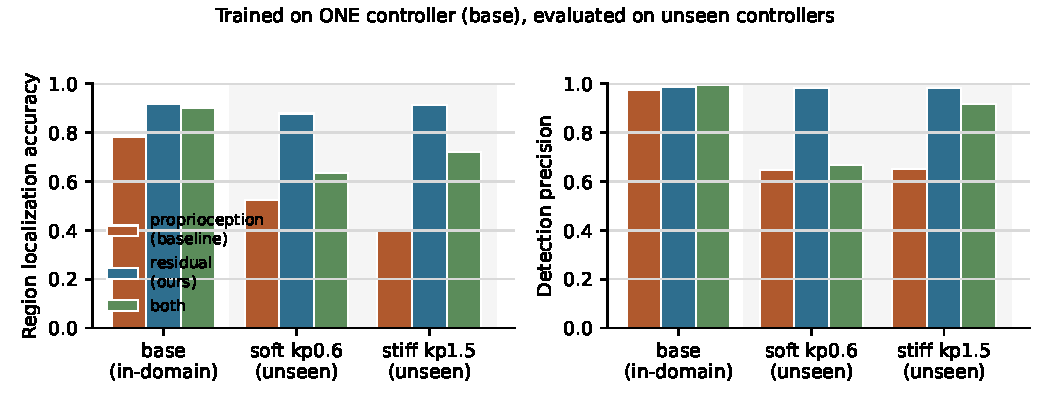
\includegraphics[width=\linewidth]{figs/fig_gap.pdf}
\caption{Cross-controller transfer (leave-one-out over 7 controllers). Raw
proprioception collapses on unseen/extreme controllers; the controller-invariant
residual channel stays flat.}
\label{fig:gap}
\end{figure}

%==============================================================================
\section{A Controller-Invariant Residual Channel}
\label{sec:method}
The failure above is shortcut learning: the raw actuator torque is the most
informative single channel for contact, but its distribution is set by the
controller, so a model that leans on it overfits the controller. We supply
instead a channel that carries the same contact information but is invariant to
the control law.

The rigid-body equation of motion is
\begin{equation}
\mathbf{M}(\mathbf{q})\ddot{\mathbf{q}} + \mathbf{c}(\mathbf{q},\dot{\mathbf{q}})
 = \boldsymbol{\tau}_{\mathrm{act}} + \boldsymbol{\tau}_{\mathrm{passive}}
   + \boldsymbol{\tau}_{\mathrm{con}} + \tauext ,
\end{equation}
where $\mathbf{c}$ collects Coriolis, centrifugal and gravity terms,
$\boldsymbol{\tau}_{\mathrm{act}}$ is the actuator torque,
$\boldsymbol{\tau}_{\mathrm{con}}=\mathbf{J}_c^{\!\top}\mathbf{f}_c$ is the
constraint (ground-reaction) force, and $\tauext=\mathbf{J}^{\!\top}\Fext$ is the
external generalized force we care about. Solving for the external term,
\begin{equation}
\label{eq:resid}
\hat{\tauext} = \mathbf{M}(\mathbf{q})\ddot{\mathbf{q}} + \mathbf{c}(\mathbf{q},\dot{\mathbf{q}})
   - \boldsymbol{\tau}_{\mathrm{act}} - \boldsymbol{\tau}_{\mathrm{passive}}
   - \boldsymbol{\tau}_{\mathrm{con}} ,
\end{equation}
gives, on the $29$ actuated joints, an estimate of the external joint torque that
depends only on measured motion
($\mathbf{q},\dot{\mathbf{q}},\ddot{\mathbf{q}}$), the measured actuator torque,
and the known model --- \emph{not} on how $\boldsymbol{\tau}_{\mathrm{act}}$ was
chosen. We feed this $29$-dim vector, windowed over $6$ steps, as an additional
input channel. Empirically $\|\hat{\tauext}\|\approx 0$ in contact-free stance
regardless of the gains and grows with the applied force, exactly the invariance
we want. We evaluate three input configurations: \emph{proprioception} (the
$320$-dim raw window; the baseline), \emph{residual} (the $29$-dim channel from
Eq.~\ref{eq:resid} alone), and \emph{both} (concatenated).

%==============================================================================
\section{Experiments}
\label{sec:exp}

\subsection{The residual channel closes the gap robustly}
\label{sec:robust}
Table~\ref{tab:main} gives the central result over the seven-controller
leave-one-out study. The residual channel is the robust winner: worst-case region
accuracy $0.91$ and mean $0.93$, with detection precision $0.97$--$0.99$ on
\emph{every} held-out controller including the extreme-soft and extreme-stiff
extrapolations, where raw proprioception falls to $0.42$/$0.47$. The ``both''
configuration is best \emph{in-domain} (e.g.\ $0.97$ on central controllers, as it
has the richest signal) but partially re-inherits the proprioception shortcut on
extreme controllers (worst-case $0.78$, precision $0.67$), confirming that the raw
torque channel is what breaks transfer. Controller randomization helps every
input (it lifts proprioception from single-controller $0.40$ to $0.70$), but even
with six training controllers raw proprioception trails the residual, which is
essentially unchanged by randomization --- the physics channel, not a bigger
training set, is what buys plug-and-play.

\begin{table}[t]
\centering
\caption{Cross-controller robustness (leave-one-out over 7 controllers, train on
6 / eval on the unseen one). Worst-case and mean over the 7 held-out controllers.}
\label{tab:main}
\small
\begin{tabular}{lcccc}
\toprule
input & worst regAcc & mean regAcc & worst prec & mean prec \\
\midrule
proprioception   & 0.417 & 0.653 & 0.53 & 0.80 \\
\textbf{residual (ours)} & \textbf{0.905} & \textbf{0.931} & \textbf{0.97} & \textbf{0.99} \\
both             & 0.777 & 0.897 & 0.67 & 0.88 \\
\bottomrule
\end{tabular}
\end{table}

\begin{figure}[t]
\centering
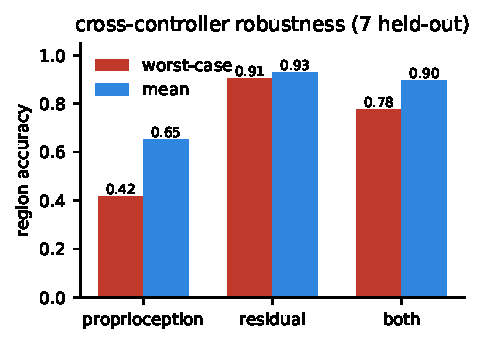
\includegraphics[width=0.92\linewidth]{figs/fig_robust.pdf}
\caption{Worst-case vs.\ mean cross-controller region accuracy over 7 held-out
controllers. The residual channel raises the worst case from $0.42$ to $0.91$.}
\label{fig:robust}
\end{figure}

\subsection{The residual also solves the legs}
\label{sec:legs}
Leg contacts are the classic hard case for proprioceptive estimation: in double
support the feet are planted, and an external leg force is partly absorbed by the
ground reaction, \emph{masking} it in the raw joint signals. Breaking down
per-region recall (Table~\ref{tab:region}, Fig.~\ref{fig:region}) shows raw
proprioception localizes arms well ($0.80$) but legs poorly ($0.56$) and trunk
worse ($0.43$). The residual channel raises legs to $0.89$ --- near arm level ---
and trunk to $0.86$. The reason is structural: Eq.~\ref{eq:resid} explicitly
subtracts the ground reaction $\boldsymbol{\tau}_{\mathrm{con}}$, removing exactly
the stance-masking term that hides leg forces. A single physics channel thus
addresses both plug-and-play transfer and leg observability.

\begin{table}[t]
\centering
\caption{Per-region recall (cross-controller, 7-fold leave-one-out average).}
\label{tab:region}
\small
\begin{tabular}{lccccc}
\toprule
input & arms & \textbf{legs} & trunk \\
\midrule
proprioception & 0.80 & 0.56 & 0.43 \\
\textbf{residual (ours)} & \textbf{0.98} & \textbf{0.89} & \textbf{0.86} \\
\bottomrule
\end{tabular}
\end{table}

\begin{figure}[t]
\centering
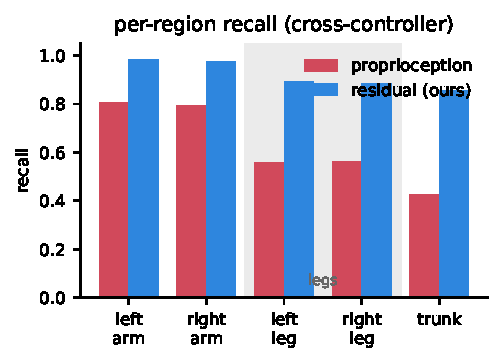
\includegraphics[width=0.92\linewidth]{figs/fig_region.pdf}
\caption{Per-region recall. The residual channel rescues the legs (and trunk) by
removing stance masking, closing the gap to the arms.}
\label{fig:region}
\end{figure}

\subsection{Making the residual hardware-realizable}
\label{sec:realize}
Of the terms in Eq.~\ref{eq:resid}, the mass matrix, bias, actuator torque and
passive forces are all computable on hardware from encoders, a model, and motor
currents; the \emph{only} simulation-privileged term is the ground reaction
$\boldsymbol{\tau}_{\mathrm{con}}$. We quantify the reliance on it in two steps.

\textbf{Without any ground-reaction term} (drop $\boldsymbol{\tau}_{\mathrm{con}}$
entirely; fully proprioception-realizable), the residual on contact-free links is
unchanged, so the \emph{arms} remain fully controller-invariant at $0.94$
(Table~\ref{tab:realize}); the legs and trunk, now contaminated by the unremoved
ground reaction, fall to $0.62$ and $0.42$. The upper-body plug-and-play claim is
thus realizable with \emph{no} extra sensing.

\textbf{With a foot ground-reaction estimate} --- what a foot F/T sensor or a
floating-base momentum observer~\cite{deluca2006momentum,mobnet} provides --- the
legs are recovered. We model an imperfect estimate as
$\hat{\boldsymbol{\tau}}_{\mathrm{con}}=\boldsymbol{\tau}_{\mathrm{con}}+\alpha\,\boldsymbol{\epsilon}$,
$\boldsymbol{\epsilon}\!\sim\!\mathcal{N}(0,\sigma_{\mathrm{GRF}})$, and sweep the
relative error $\alpha$ (Fig.~\ref{fig:grfnoise}). At $\alpha\!=\!0$ (perfect
estimate) legs return to $0.92$; degradation is graceful --- $0.84$ at $10\%$
error, $0.79$ at $25\%$, $0.73$ at $50\%$ --- with the arms unaffected throughout
($0.97$). Since a foot F/T sensor typically has well under $10\%$ error, the leg
result is realizable on any humanoid with foot force sensing, and robust to its
noise; the trunk is the most estimate-sensitive region.

\begin{table}[t]
\centering
\caption{Realizability of the residual. ``full'' subtracts the (privileged)
ground reaction; ``realizable'' drops it (proprioception-only).}
\label{tab:realize}
\small
\begin{tabular}{lcccc}
\toprule
residual & arms & \textbf{legs} & trunk & worst-case regAcc \\
\midrule
full (privileged GRF) & 0.98 & 0.89 & 0.86 & 0.905 \\
realizable (no GRF)   & 0.94 & 0.62 & 0.42 & 0.586 \\
\bottomrule
\end{tabular}
\end{table}

\begin{figure}[t]
\centering
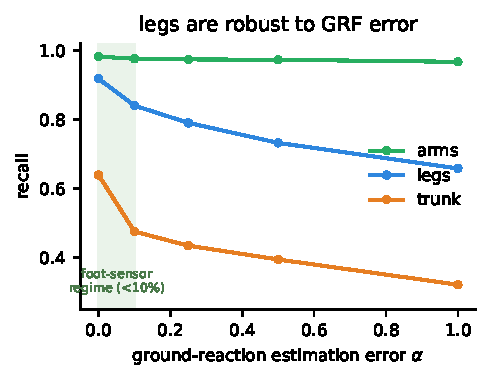
\includegraphics[width=0.92\linewidth]{figs/fig_grfnoise.pdf}
\caption{Legs are robust to ground-reaction estimation error: recall degrades
gracefully with $\alpha$ while the arms are unaffected. A realistic foot-sensor
error ($<10\%$) keeps legs near $0.86$--$0.89$.}
\label{fig:grfnoise}
\end{figure}

%==============================================================================
\section{Discussion and Limitations}
\label{sec:limits}
\textbf{``Different controller'' is emulated by gain scaling.} We did not train
several distinct networks; we scaled PD gains, which shifts the actuator-torque
distribution --- the channel that matters --- but is a smaller perturbation than a
genuinely different policy. Our measured gap is therefore a \emph{lower bound},
and confirming that the residual transfers across truly different trained
controllers is the necessary next step.

\textbf{Ground reaction on hardware.} The full residual reads
$\boldsymbol{\tau}_{\mathrm{con}}$ from the simulator; on hardware it comes from a
foot F/T sensor or a floating-base momentum
observer~\cite{deluca2006momentum,mobnet}. Sec.~\ref{sec:realize} bounds the
impact: the upper body needs nothing extra, and the legs tolerate substantial
ground-reaction error, but a hardware demonstration remains future work.

\textbf{Scope.} All results are in simulation, at $5$-region granularity, with
sustained forces; we have not evaluated per-link wrench regression (matching
SixthSense's output), force-magnitude accuracy, walking/dynamic tracking, or a
real robot. These are the axes to widen before claims of practical deployment.

%==============================================================================
\section{Conclusion}
We asked whether a proprioceptive whole-body contact estimator can serve as a
plug-and-play module across the many controllers a humanoid runs. The standard
end-to-end recipe does not transfer --- a different controller shifts the
actuator-torque distribution the estimator depends on, collapsing accuracy and
precision. A controller-invariant residual channel, recovered from the equation of
motion, restores transfer robustly across a wide range of controllers, and as a
by-product removes the double-support stance masking that makes legs hard, raising
leg recall to arm level. The channel is hardware-realizable: the upper body needs
only proprioception, and the legs need only a foot ground-reaction estimate, to
which they are robust. A genuine plug-and-play contact-sensing module for
humanoids therefore runs not through a bigger passive estimator, but through the
right, controller-agnostic representation of the external force.

\bibliographystyle{IEEEtran}
\bibliography{references}

\end{document}
